\documentclass[12pt,a4paper]{article}

\usepackage[T1]{fontenc}
\usepackage[utf8]{inputenc}
\usepackage[brazil]{babel} % Alterado de brazilian para brazil

\AtBeginDocument{%
	\renewcommand{\figurename}{Figura}%
	\renewcommand{\tablename}{Tabela}%
	\renewcommand{\listfigurename}{Lista de Figuras}%
	\renewcommand{\listtablename}{Lista de Tabelas}%
	\renewcommand{\contentsname}{Sumário}%
	\renewcommand{\today}{\number\day\ de \ifcase\month\or
		janeiro\or fevereiro\or março\or abril\or maio\or junho\or
		julho\or agosto\or setembro\or outubro\or novembro\or dezembro\fi
		\ de \number\year}
}
	
\usepackage{helvet}
\renewcommand{\familydefault}{\sfdefault}

\usepackage[a4paper,margin=2.5cm]{geometry}
\usepackage{setspace}
\usepackage{enumitem}
\usepackage{array}
\usepackage{tabularx}
\usepackage{booktabs}	
\usepackage{titlesec}
\usepackage{tocloft}
\usepackage{fancyhdr}
\usepackage{hyperref}
\usepackage{ragged2e}
\usepackage{amsmath}
\usepackage{graphicx}
\usepackage{float}

\hypersetup{
	colorlinks=true,
	linkcolor=black,
	urlcolor=black,
	pdftitle={[Gerador de números Pseudo-Aleatórioscom não repetição baseada em detecção por Handshaking]: Relatório Final de Projeto Fase II},
	pageanchor=false
}

\setlength{\parindent}{0pt}
\setlength{\parskip}{0pt}
\setlist[itemize]{topsep=2pt,itemsep=4pt,parsep=0pt,partopsep=0pt}
\setlist[itemize,2]{topsep=2pt,itemsep=3pt}

\pagestyle{fancy}
\fancyhf{}
\fancyfoot[R]{\thepage}
\renewcommand{\headrulewidth}{0pt}
\renewcommand{\footrulewidth}{0pt}
\fancypagestyle{plain}{\fancyhf{}\fancyfoot[R]{\thepage}\renewcommand{\headrulewidth}{0pt}\renewcommand{\footrulewidth}{0pt}}

\titleformat{\section}
{\normalfont\bfseries\fontsize{24}{28}\selectfont}
{\thesection.}
{0.45em}
{}
\titlespacing*{\section}{0pt}{0pt}{0.65em}

\renewcommand{\contentsname}{Sumário}
\renewcommand{\cfttoctitlefont}{\bfseries\fontsize{24}{28}\selectfont}
\renewcommand{\cftaftertoctitle}{\vskip 1.0em}
\setlength{\cftbeforesecskip}{0.55em}
\renewcommand{\cftsecfont}{\normalsize}
\renewcommand{\cftsecpagefont}{\normalsize}
\setlength{\cftsecindent}{1.5em}
\setlength{\cftsecnumwidth}{1.8em}
\renewcommand{\cftdotsep}{1.2}
\renewcommand{\cftsecleader}{\cftdotfill{\cftdotsep}}

\newcolumntype{Y}{>{\RaggedRight\arraybackslash}X}
\newcolumntype{M}[1]{>{\RaggedRight\arraybackslash}m{#1}}

\newcommand{\templatefigure}[3][0.9\textwidth]{%
	\begin{figure}[H]
		\centering
		\IfFileExists{#2}{%
			\fbox{\includegraphics[width=#1]{#2}}%
		}{%
			\fbox{\parbox[c][0.22\textheight][c]{0.82\textwidth}{\centering\small Arquivo de imagem não encontrado\\\texttt{\detokenize{#2}}}}%
		}%
		\caption{#3}
	\end{figure}
}

\begin{document}
	\selectlanguage{brazil} 
	
	% -----------------------------------------------------------------------------
	% CAPA
	% -----------------------------------------------------------------------------
	\thispagestyle{fancy}
	\vspace*{1.3cm}
	
	{\bfseries\fontsize{24}{28}\selectfont Gerador de números pseudo-aleatórios com detecção de não repetição baseada em Handshaking: Relatório Final de\\Projeto Fase II\par}
	
	\vspace{2.2cm}
	
	{\large\textbf{Integrante(s):} Matheus Grossi\par}
	\vspace{1.2cm}
	{\large\textbf{Data:} \today\par}
	\vspace{1.2cm}
	{\large\textbf{Tecnologia Alvo:} SkyWater 130nm / FPGA Xilinx Spartan-3E (90nm)\par}
	
	\clearpage
	
	% -----------------------------------------------------------------------------
	% SUMÁRIO
	% -----------------------------------------------------------------------------
	\thispagestyle{fancy}
	\tableofcontents
	
	\clearpage
	\setcounter{page}{1}
	
	% -----------------------------------------------------------------------------
	% 1. INTRODUÇÃO E ESPECIFICAÇÃO
	% -----------------------------------------------------------------------------
	\section{Introdução e Especificação}
	
	\begin{itemize}[leftmargin=1.4em]
		\item \textbf{Resumo Executivo:} Este projeto consiste na implementação em Verilog de um Gerador de Números Pseudoaleatórios (PRNG). O sistema foi projetado para gerar números de 3 bits (faixa de 0 a 7) utilizando 4 sementes (seeds) distintas baseadas em tabelas de permutação.
		
		\vspace{0.5cm}
		
		\item \textbf{Arquitetura do Sistema:} 
		
		\begin{figure}[H]
			\centering
			\IfFileExists{../../diagrams/topview/topview.png}{%
				\fbox{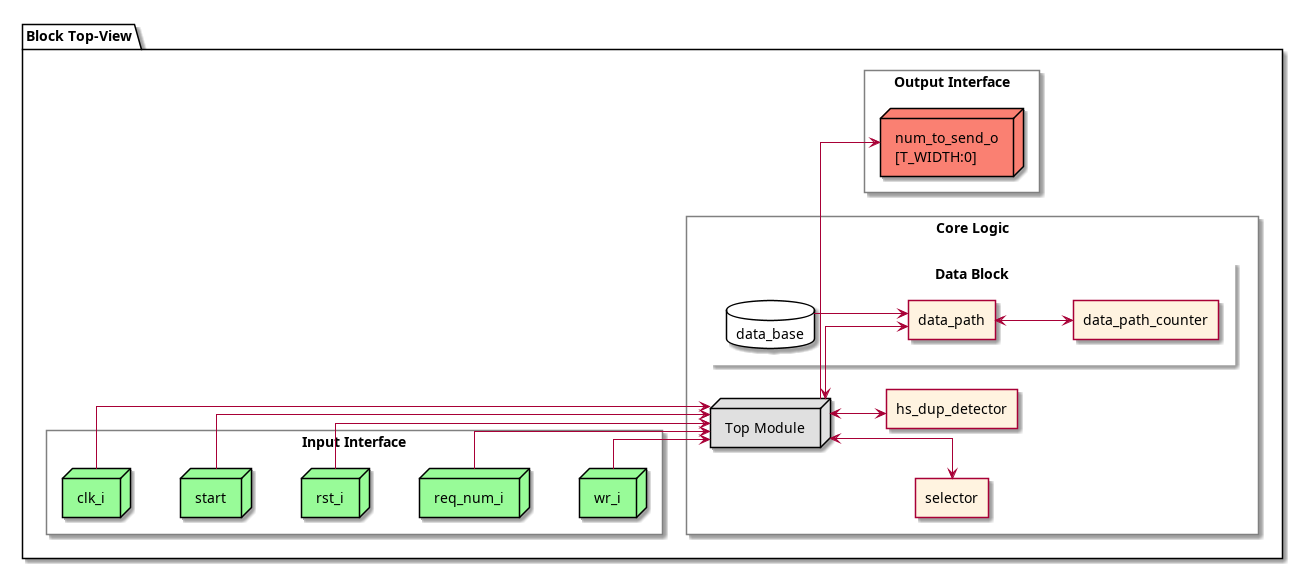
\includegraphics[width=0.94\textwidth]{../../diagrams/topview/topview.png}}%
			}{%
				\fbox{\parbox[c][0.22\textheight][c]{0.82\textwidth}{\centering\small Arquivo de imagem não encontrado\\\texttt{../../diagrams/topview/topview.png}}}%
			}
			\caption{Representação em blocos da arquitetura do sistema}
			\label{fig:rtl-topview}
		\end{figure}
		
		\item \textbf{Tabela de Interfaces:} 
		
		\begin{table}[H]
			\centering
			\small
			\begin{tabularx}{\textwidth}{|M{3.0cm}|M{1.2cm}|M{1.4cm}|Y|}
				\hline
				\textbf{Sinal} & \textbf{Dir.} & \textbf{Bits} & \textbf{Descrição funcional} \\
				\hline
				\texttt{clk\_i} & I & 1 & Clock principal do sistema. \\
				\hline
				\texttt{rst\_i} & I & 1 & Reset assíncrono ativo em nível baixo. \\
				\hline
				\texttt{req\_num\_i} & I & 1 & Requisição de geração de um novo número pseudoaleatório. \\
				\hline
				\texttt{wr\_i} & I & 1 & Confirmação de escrita/aceite; ao ser ativado, o valor válido é salvo no histórico. \\
				\hline
				\texttt{num\_to\_send\_o} & O & 3 & Saída de dado pseudoaleatório validado pelo detector de duplicatas. \\
				\hline
			\end{tabularx}
			\caption{Interface funcional do módulo de topo \texttt{rng\_top}.}
		\end{table}
		
		
		\item \textbf{Conformidade com Protocolos:} Para a detecção de duplicidade há um sistema iterno de handshaking para detectar se os valores que chegam já são existentes no banco de memória e caso sejam são descartados e solicitam uma nova amostra.
		
		\vspace{0.5cm}
		
		\item \textbf{Mapa de Registradores:} Tabela detalhando endereços, permissões (R/W) e funções de cada bit.
		
		\begin{table}[H]
			\centering
			\small
			\begin{tabularx}{\textwidth}{|M{3.0cm}|M{1.2cm}|M{1.4cm}|Y|}
				\hline
				
				\textbf{Nome} & \textbf{Tipo.} & \textbf{Bits} & \textbf{Descrição funcional} \\
				
				\hline
				
				\texttt{ram\_0} & reg. & 3 & 1°  Bit do barramento de memória \\
				
				\hline
				
				\texttt{ram\_1} & reg. & 3 & 2°  Bit do barramento de memória \\
				
				\hline
				
				\texttt{ram\_2} & reg. & 3 & 3°  Bit do barramento de memória \\
				
				\hline
				
				\texttt{ram\_3} & reg. & 3 & 4°  Bit do barramento de memória \\
				
				\hline
				
				\texttt{ram\_4} & reg. & 3 & 5°  Bit do barramento de memória \\
				
				\hline
				
				\texttt{ram\_5} & reg. & 3 & 6°  Bit do barramento de memória \\
				
				\hline
				
				\texttt{ram\_6} & reg. & 3 & 7°  Bit do barramento de memória \\
				
				\hline
				
				\texttt{ram\_7} & reg. & 3 & 8°  Bit do barramento de memória \\
				
				\hline
				
			\end{tabularx}
			
			\caption{Registradores internos do validador de handshaking implementado na bancada UVM.}
		\end{table}
		
	\end{itemize}
	
	\clearpage
	
	% -----------------------------------------------------------------------------
	% 2. IMPLEMENTAÇÃO RTL
	% -----------------------------------------------------------------------------
	
	\section{Implementação RTL}
	
	A implementação RTL do bloco foi desenvolvida em Verilog com foco em portabilidade entre FPGA e ASIC. O circuito gera valores pseudoaleatórios de \textbf{3 bits}, na faixa de 0 a 7, e incorpora um mecanismo de \textbf{não repetição} baseado em histórico interno e protocolo de handshaking. A arquitetura foi organizada de forma hierárquica para separar geração de candidatos, seleção de sementes, controle temporal e detecção de duplicatas.
	
	\subsection*{Estratégia de design}
	
	O módulo de topo é o \texttt{rng\_top}, responsável por integrar os sub-blocos funcionais e expor a interface externa do sistema. A hierarquia descrita na documentação-base é composta pelos seguintes blocos:
	
	\vspace{0.5cm}
	\begin{itemize}[leftmargin=1.4em]
		\item \textbf{\texttt{rng\_top}:} integra controle, caminho de dados e lógica de não repetição;
		\item \textbf{\texttt{rng\_selector}:} seleciona uma entre \textbf{4 seeds} por meio de um contador \textit{free-running}, produzindo o índice da tabela de permutação ativa;
		\item \textbf{\texttt{rng\_data\_path}:} multiplexa o valor numérico candidato com base na seed selecionada e na posição corrente da sequência;
		\item \textbf{\texttt{rng\_data\_path\_counter}:} contador cíclico de 3 bits que percorre as posições das tabelas internas;
		\item \textbf{\texttt{rng\_hs\_dup\_detector}:} armazena o histórico dos valores já aceitos, compara o candidato atual com esse histórico e rejeita repetições.
	\end{itemize}
	
	\subsection*{Fluxo funcional do RTL}
	
	O funcionamento do bloco ocorre em etapas bem definidas, mantendo a coerência entre geração pseudoaleatória e aceite do dado pela interface de saída:
	
	\begin{enumerate}[leftmargin=1.6em]
		\item \textbf{Reset:} o sinal \texttt{rst\_i} limpa a memória do detector de duplicatas e reinicializa o estado operacional do bloco;
		\item \textbf{Seleção de seed:} o \texttt{rng\_selector} escolhe a tabela de permutação ativa a partir de um contador interno;
		\item \textbf{Geração do candidato:} o \texttt{rng\_data\_path} produz um valor de 3 bits com base na combinação entre seed e índice atual;
		\item \textbf{Validação:} o \texttt{rng\_hs\_dup\_detector} compara o candidato com o histórico armazenado; valores repetidos são descartados e o circuito busca a próxima combinação válida;
		\item \textbf{Handshake e armazenamento:} quando o consumidor confirma a leitura por \texttt{wr\_i}, o valor aceito é gravado no histórico de não repetição.
	\end{enumerate}
	
	Esse fluxo mostra que a unicidade das saídas não depende apenas da escolha da seed, mas da cooperação entre caminho de dados, lógica de comparação e protocolo de aceite.
	
	\subsection*{Parâmetros e escalabilidade}
	
	Embora o sistema não seja totalmente parametrizável devido à limitações nas criações do barramento de memória ainda sim trabalhei da forma mais modular possível:
	
	\renewcommand{\arraystretch}{1.4}
	\setlength{\tabcolsep}{5pt}
	
	\begin{table}[H]
		\centering
		\small
		\begin{tabularx}{\textwidth}{|M{2.6cm}|M{2.5cm}|Y|}
			\hline
			\textbf{Parâmetro} & \textbf{Valor} & \textbf{Função no RTL} \\
			\hline
			\texttt{WIDTH} & 3 & Largura do dado pseudoaleatório, correspondente aos valores de 0 a 7. \\
			\hline
			\texttt{T\_WIDTH} & \texttt{WIDTH-1} & Ajuste auxiliar para declaração de vetores e barramentos. \\
			\hline
			\texttt{SEED\_TOT\_NUMB} & 12 & Quantidade total de números organizados nas sementes e tabelas internas. \\
			\hline
			\texttt{COUNT\_WIDTH} & \texttt{\$clog2(...)} & Largura calculada para os contadores associados ao avanço de estados e sequências. \\
			\hline
		\end{tabularx}
		\caption{Parâmetros estruturais descritos na documentação de especificação.}
	\end{table}
	
	\subsection*{Controle e FSMs}
	
	O bloco possui um sistema de máquina de estados complexa que pode ser descrita melhor abaixo:
	
	\vspace{0.5cm}
	
	\begin{itemize}[leftmargin=1.4em]
		
		\item Reset: Ao iniciar, o sistema deve ser resetado (\texttt{rst\_i}). Isso limpa a memória do detector de duplicatas, reinicia os contadores e define o estado inicial da FSM.
		
		\item Seleção de Seed: O módulo \texttt{rng\_selector} utiliza o clock para incrementar um contador interno. O momento da ativação define qual das 4 tabelas de permutação será usada para a geração atual.
		
		\item Geração e Validação (Loop Interno): O \texttt{rng\_data\_path} fornece um número candidato baseado na seed e no contador sequencial. O \texttt{rng\_hs\_dup\_detector} verifica se este número existe na memória interna (\texttt{mem}).
		
		\item Se existir (Duplicata): O detector ativa o sinal interno \texttt{req\_new\_num\_o}. Isso força o sistema a descartar o número atual e buscar o próximo imediatamente na tabela.
		
		\item Se não existir (Único): O número é disponibilizado em \texttt{num\_to\_send\_o}.
		
		\item Confirmação de Leitura: O usuário/sistema externo deve enviar o sinal \texttt{wr\_i} para confirmar o uso do número. Isso instrui o detector a armazenar o valor atual na memória de histórico, impedindo que ele seja gerado novamente até que o buffer seja limpo ou reiniciado.
		
	\end{itemize}
	
	\templatefigure[0.65\textwidth]{../../diagrams/fsm/fsm.png}{Diagrama de estados da FSM.}
	
	
	Em termos práticos, a sequência de operação pode ser interpretada como um fluxo de estados implícitos:
	
	\vspace{0.5cm}
	
	\begin{itemize}[leftmargin=1.4em]
		\item \textbf{Inicialização}, após reset;
		\item \textbf{Seleção e geração}, quando um novo candidato é produzido;
		\item \textbf{Comparação}, quando o candidato é confrontado com o histórico armazenado;
		\item \textbf{Aceite}, quando \texttt{wr\_i} confirma a transferência de um valor válido.
	\end{itemize}
	
	\vspace{0.5cm}
	
	Abaixo há uma ilustração pré-projeto do comportamento esperado do circuito:
	
	\templatefigure[0.85\textwidth]{../../diagrams/timing/timing.png}{Diagrama de temporização do protocolo de operação do bloco.}
	
	\clearpage
	
	% -----------------------------------------------------------------------------
	% 3. ESTRATÉGIA DE VERIFICAÇÃO E RESULTADOS
	% -----------------------------------------------------------------------------
	\section{Estratégia de Verificação e Resultados}
	
	A estratégia de verificação do bloco foi estruturada em torno de uma bancada UVM executada com Verilator e analisada com apoio do GTKWave. O foco da campanha foi validar o protocolo de handshaking do gerador pseudo-aleatório, a captura correta das amostras produzidas pelo DUT e a consolidação dos resultados observados no scoreboard.
	
	\subsection*{Visão geral da bancada}
	
	\begin{itemize}[leftmargin=1.4em]
		\item \textbf{Bloco verificado:} gerador de números pseudo-aleatórios de 3 bits com não repetição (RNG).
		\item \textbf{Versão da verificação:} 1.0.
		\item \textbf{Responsável pela verificação:} Matheus Grossi.
		\item \textbf{Ferramentas utilizadas:} UVM, Verilator e GTKWave.
		\item \textbf{Período da campanha:} 24/02/2026 a 10/03/2026.
	\end{itemize}
	
	\templatefigure[0.2\textwidth]{../doc_verif/UVM.png}{Lista de itens que compõem a bancada.}
	
	\subsection*{Objetivos da verificação}
	
	O objetivo da verificação foi assegurar os seguintes pontos funcionais e estruturais:
	
	\vspace{0.5cm}
	
	\begin{itemize}[leftmargin=1.4em]
		\item O protocolo de solicitação e aceite do bloco, por meio dos sinais \texttt{req\_num\_i} e \texttt{wr\_i}, ocorre conforme o handshaking modelado na bancada;
		\item O monitor captura corretamente as amostras válidas de \texttt{num\_to\_send\_o} na presença de \texttt{wr\_i};
		\item O scoreboard consolida a sequência observada, contabiliza ocorrências e sinaliza repetições reais;
		\item O DUT é exercitado sob três faixas de temporização configuradas na sequência, com \texttt{clk\_toggle\_tu} igual a 3, 7 e 10, além de espaçamentos pseudoaleatórios entre requisições.
	\end{itemize}
	
	\subsection*{Caso de teste executado}
	
	\renewcommand{\arraystretch}{1.35}
	\setlength{\tabcolsep}{5pt}
	
	\begin{table}[H]
		\centering
		\small
		\begin{tabularx}{\textwidth}{|M{1.8cm}|Y|M{2.7cm}|Y|Y|}
			\hline
			\textbf{ID do Teste} & \textbf{Descrição} & \textbf{Sequência Principal} & \textbf{Ambiente} & \textbf{Critério de Sucesso} \\
			\hline
			\texttt{rng\_test} & Teste principal com 24 rodadas, divididas em três faixas temporais, com intervalos pseudoaleatórios entre requisições. O teste valida o handshaking, a captura das amostras pelo monitor e a consolidação da sequência observada no scoreboard. & \texttt{rng\_sequence} & \texttt{tb\_rng}, \texttt{rng\_env}, \texttt{rng\_agent}, \texttt{rng\_driver}, \texttt{rng\_monitor} e \texttt{rng\_scoreboard} & Execução completa das 24 rodadas, ausência de \texttt{uvm\_fatal}, publicação de amostras válidas pelo monitor e geração do resumo final do scoreboard com contagem consistente. \\
			\hline
		\end{tabularx}
	\end{table}
	
	\subsection*{Resultados obtidos}
	
	\begin{itemize}[leftmargin=1.4em]
		\item \textbf{Total de sequências:} 1 sequência principal, \texttt{rng\_sequence}.
		\item \textbf{Testes aprovados:} 1 teste estrutural previsto pela bancada.
		\item \textbf{Testes com falha explícita:} 0 falhas estruturais explícitas na bancada.
	\end{itemize}
	
	\vspace{0.5cm}
	Do ponto de vista estrutural, os comportamentos esperados foram observados. A bancada verificou corretamente a liberação de reset, a execução das 24 rodadas, a variação temporal do clock por item de sequência, a publicação de amostras pelo monitor quando \texttt{wr\_i} está ativo e a consolidação das ocorrências no scoreboard.
	
	Também foi identificado um comportamento inesperado durante a verificação: uma falha no protocolo de handshaking. Após a execução de lint, os erros no RTL foram localizados e corrigidos, permitindo a continuidade da campanha de verificação com a bancada já estabilizada.
	
	\subsection*{Análise dos resultados}
	
	A bancada está organizada em UVM com agente, sequencer, driver, monitor, ambiente e scoreboard conectados de forma coerente. Por se tratar de um projeto residencial e feita em um compilador com restrições de SystemVerilog não foi feita uma cobertura mais aprofundada, para um caso de projeto comercial desse bloco recomenda-se uma abordagem mais densa de verificação.
	
	\subsection*{Cobertura de verificação}
	
	\templatefigure[0.96\textwidth]{../doc_verif/coverage_list.png}{Lista do relatório de cobertura da bancada.}
	
	A cobertura atualmente obtida é predominantemente \textbf{estrutural e observacional}. O monitor coleta amostras válidas da saída e o scoreboard resume histograma, quantidade de valores únicos, duplicatas reais e sequência observada. Entretanto, ainda não há métricas formais de cobertura para:
	
	\vspace{0.5cm}
	
	\begin{itemize}[leftmargin=1.4em]
		\item todos os valores possíveis de 3 bits;
		\item a exaustão completa do conjunto sem repetição;
		\item as transições entre estados internos do DUT;
		\item cenários de erro ou de violação de protocolo.
	\end{itemize}
	
	\subsection*{Limitações observadas}
	
	Foi registrado que o desenvolvimento da bancada ainda pode evoluir em profundidade metodológica. Em particular, a ausência de um modelo de referência, de cobertura funcional e de checagens mandatórias para cenários negativos indica espaço para amadurecimento da estratégia de verificação nas próximas iterações.
	
	\subsection*{Conclusão da verificação}
	
	A bancada UVM do bloco RNG foi concluída com sucesso e mostrou-se apta para uso em simulação e depuração do DUT. Como próximos avanços naturais, a campanha pode incorporar cobertura funcional, um modelo de referência explícito e critérios de falha mais rigorosos para o requisito de não repetição.
	
	
	\clearpage
	
	% -----------------------------------------------------------------------------
	% 4. SÍNTESE LÓGICA E RESULTADOS PPA
	% -----------------------------------------------------------------------------
	\section{Síntese Lógica e Resultados PPA}
	
	Neste projeto foram adotados dois cenários: uma síntese direcionada a FPGA para inspeção estrutural do hardware e um fluxo ASIC baseado no ambiente \textit{Librelane}, com mapeamento tecnológico para a biblioteca de \textit{standard cells} \texttt{sky130\_fd\_sc\_hd} do PDK SkyWater 130 nm. Como o projeto foi tratado como prova de conceito e não como candidato imediato a \textit{tape-out}, as restrições temporais aplicadas foram genéricas, de modo que os resultados de performance e potência devem ser interpretados como preliminares e dependentes de refinamento posterior. 
	
	\templatefigure[0.65\textwidth]{../../diagrams/soc_view.png}{Vista pós-síntese do SoC apresentada na documentação-base.}
	
	\subsection*{Considerações de ASIC}
	
	Esse bloco possui 3 pontos importantes a mencionar:
	
	\begin{itemize}[leftmargin=1.4em]
		\vspace{0.5cm}
		\item \textbf{Domínio de clock único:} o bloco opera a partir do sinal \texttt{clk\_i}, sem múltiplos domínios de clock;
		\item \textbf{Reset bem definido:} o sinal \texttt{rst\_i} é assíncrono e ativo em nível baixo, permitindo limpeza imediata do histórico e reinicialização do fluxo operacional;
		\item \textbf{Estilo sintetizável:} a separação entre blocos de dados, seleção e armazenamento favorece uma descrição RTL compatível com síntese e reduz o risco de \textit{latches} indesejados, desde que a codificação combinacional mantenha atribuições completas.
		\vspace{0.5cm}
	\end{itemize}
	
	Além disso, a existência de um contador, tabelas de permutação e memória de histórico torna o projeto naturalmente adequado a estudos comparativos entre FPGA e ASIC, especialmente em área, temporização e custo de implementação do mecanismo de não repetição.
	
	A síntese baseada em FPGA foi feita com base nas constrainsts genéricas do Basys2 e os resultados obtidos podem ser vistos abaixo:
	
	\begin{figure}[H]
		\centering
		\fbox{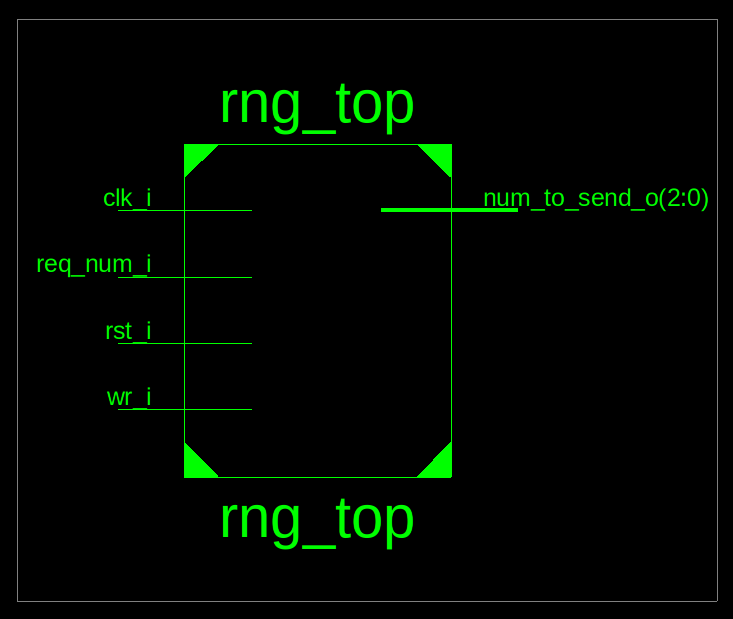
\includegraphics[width=0.65\textwidth]{../../diagrams/fpga_post_synth/top_view.png}}
		\caption{Visão de Topo do Circuito (Síntese)} 
	\end{figure}
	
	% Vistas Explodidas Separadas Verticalmente
	\begin{figure}[H]
		\centering
		\fbox{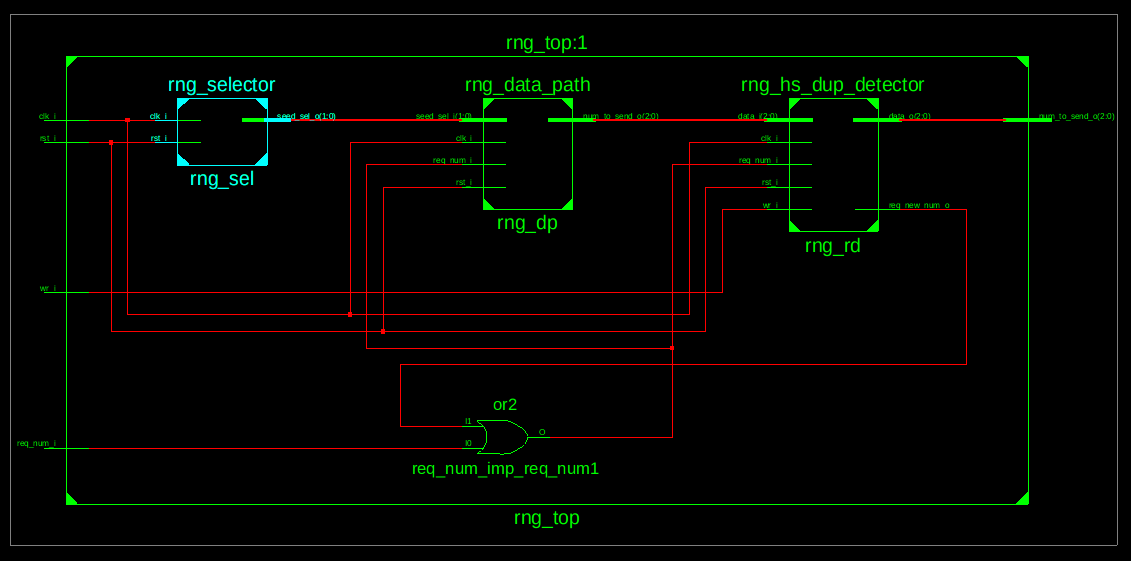
\includegraphics[width=0.65\textwidth]{../../diagrams/fpga_post_synth/xplode_view_pt1.png}}
		\caption{Vista Explodida 1}
	\end{figure}
	
	\begin{figure}[H]
		\centering
		\fbox{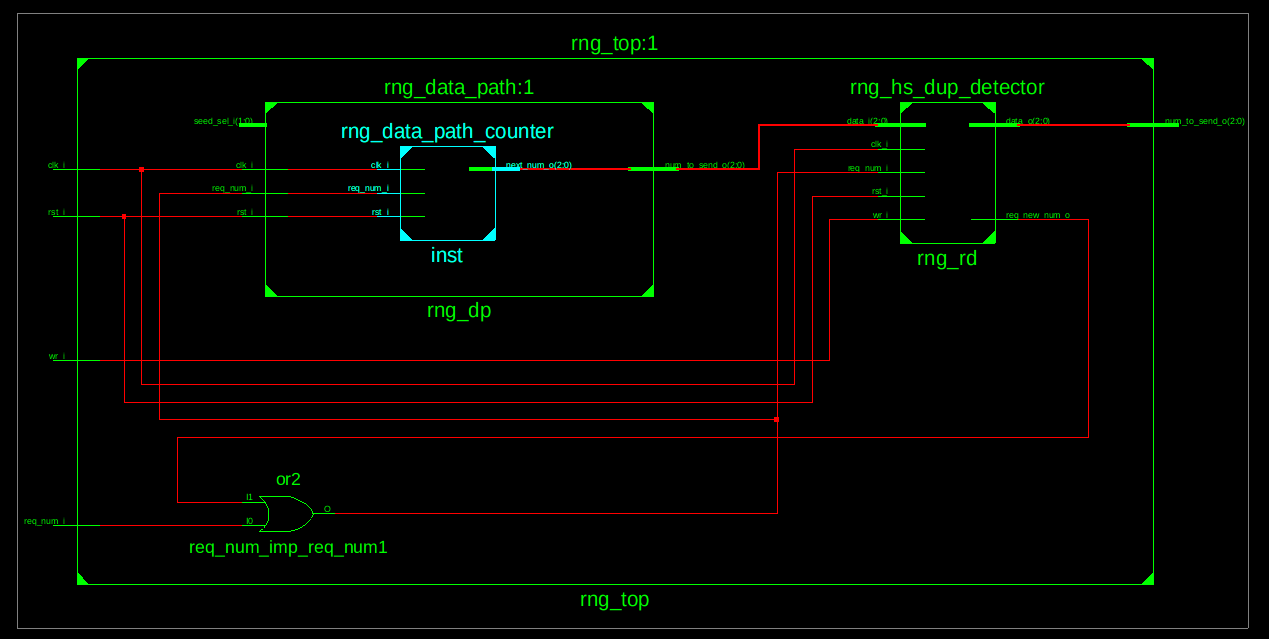
\includegraphics[width=0.65\textwidth]{../../diagrams/fpga_post_synth/xplode_view_pt2.png}}
		\caption{Vista Explodida 2}
	\end{figure}
	
	\begin{figure}[H]
		\centering
		\fbox{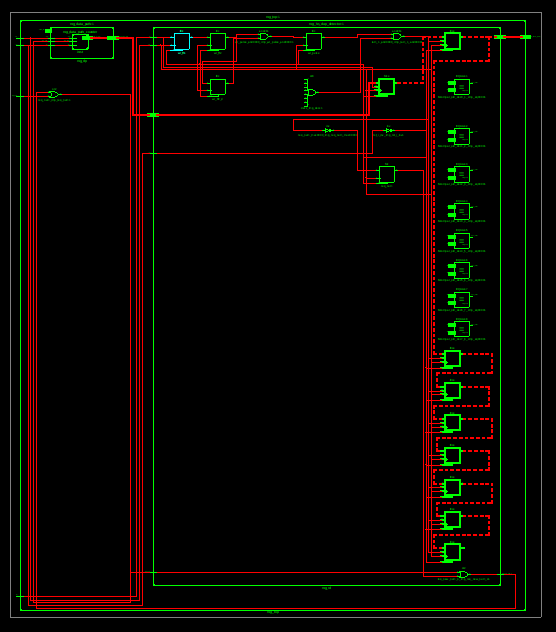
\includegraphics[width=0.85\textwidth]{../../diagrams/fpga_post_synth/xplode_view_pt3.png}}
		\caption{Vista Explodida 3}
	\end{figure}
	
	\begin{figure}[H]
		\centering
		\fbox{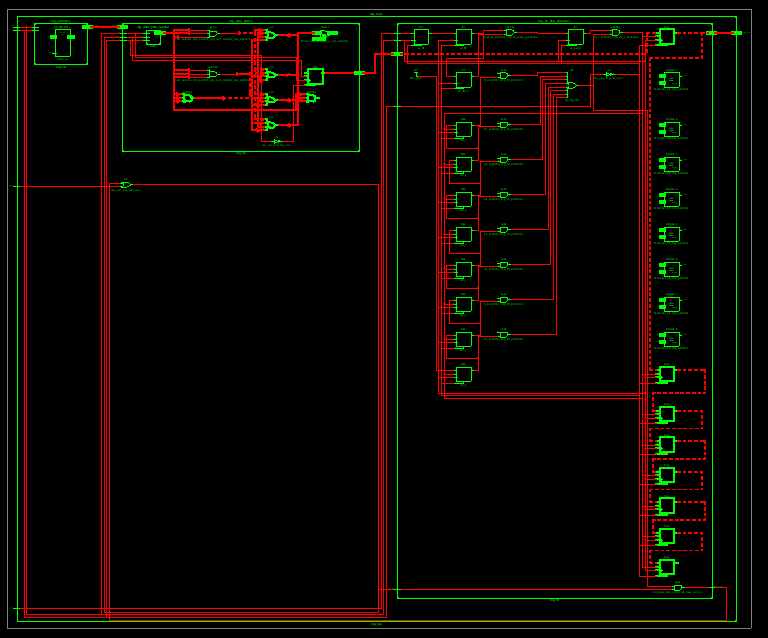
\includegraphics[width=0.85\textwidth]{../../diagrams/fpga_post_synth/xplode_view_pt4.png}}
		\caption{Vista Explodida 4}
	\end{figure}
	
	\subsection*{Fluxo de síntese adotado}
	
	No fluxo ASIC descrito no material-base, a preparação do projeto parte da criação de uma pasta dedicada dentro de \texttt{openframe\_user/openlane}, contendo um subdiretório \texttt{src} para os arquivos RTL e um arquivo \texttt{config.json} na raiz do projeto. Esse arquivo centraliza os parâmetros básicos de síntese e roteamento antes da aplicação das \textit{constraints} SDC. O documento também explicita que os ficheiros \texttt{.v} e \texttt{.sv} do projeto foram concentrados na pasta \texttt{src}, mantendo uma organização compatível com o fluxo padrão da ferramenta.
	
	\templatefigure[0.92\textwidth]{../doc_synth/org.png}{Organização da árvore de projeto.}
	
	\templatefigure[0.85\textwidth]{../doc_synth/config.png}{Configuração do arquivo \texttt{config.json} utilizado na síntese.}
	
	\subsection*{Restrições e premissas de implementação}
	
	As restrições de projeto foram mantidas em um nível genérico, sem um arquivo SDC ajustado especificamente para metas agressivas de frequência, fechamento temporal fino ou otimização direcionada a um \textit{sign-off} de produção. Essa escolha é coerente com o caráter acadêmico e exploratório do trabalho, mas impõe uma limitação importante à leitura de PPA: quaisquer conclusões quantitativas sobre frequência máxima, \textit{slack}, área física final e potência devem ser tratadas como indicativas, e não como números finais de projeto.
	
	\subsection*{Resultados da síntese lógica}
	
	A tradução do módulo \texttt{rng\_top} para nível de portas preservou a decomposição funcional apresentada nas seções anteriores, reunindo caminho de dados, seletor de sementes, detector de duplicatas e contador cíclico. O mapeamento lógico resultou em uso intensivo de multiplexadores para roteamento de dados e de portas XOR para as etapas de validação e contagem. O dado quantitativo explicitamente informado é a utilização total de \textbf{122 células lógicas}, valor que caracteriza uma implementação compacta para o porte do bloco e coerente com a simplicidade relativa do algoritmo e da interface de handshaking.
	
	\templatefigure[0.5\textwidth]{../doc_synth/stats.png}{Resumo da composição lógica do circuito apresentado na documentação de síntese.}
	
	\subsection*{Leitura dos resultados de PPA}
	
	Embora a seção original faça referência a PPA, o material fornecido não traz todos os números clássicos de \textit{Performance, Power and Area} já consolidados em formato tabular. Em particular, a documentação não explicita frequência máxima atingida, \textit{Worst Negative Slack} (WNS), área total em \textmu m\textsuperscript{2} ou equivalência em portas NAND2. Ainda assim, ela permite registrar de forma objetiva o estado atual da caracterização do bloco:
	
	
	No caso específico da potência, o texto destaca corretamente que os relatórios estáticos de síntese (como \texttt{stat.rpt} e \texttt{stat.json}) não bastam para uma estimativa dinâmica realista. Para obter \textit{dynamic power} e \textit{leakage} com maior fidelidade, o fluxo precisa incorporar dados de atividade de comutação oriundos das simulações pós-síntese, normalmente por meio de ficheiros \texttt{.vcd} gerados na pasta de \textit{waveforms} e consumidos por uma ferramenta de \textit{Power Analysis}. Assim, a caracterização energética do bloco ainda deve ser vista como pendente de fechamento metodológico.
	
	\templatefigure[0.65\textwidth]{../doc_synth/power.png}{Resumo visual das métricas de potência referenciadas no material-base.}
	
	\subsection*{Discussão técnica}
	
	Do ponto de vista de área e complexidade lógica, o resultado de 122 células sugere que o bloco possui custo de implementação modesto, o que é compatível com uma arquitetura síncrona de propósito específico e com largura de dados reduzida. Em contrapartida, a ausência de \textit{constraints} refinadas e de números temporais consolidados impede afirmar, nesta fase, qual é o limite real de desempenho do circuito em ASIC. Em outras palavras, a síntese lógica já demonstra viabilidade de implementação, mas a etapa de PPA ainda precisa ser aprofundada com relatórios temporais completos, extração pós-roteamento e análise de potência baseada em atividade.
	
	\clearpage
	
	% -----------------------------------------------------------------------------
	% 5. CONCLUSÃO E LIÇÕES APRENDIDAS
	% -----------------------------------------------------------------------------
	\section{Conclusão e Lições Aprendidas}
	
	\begin{itemize}[leftmargin=1.4em]
		\item Muitas dificuldades surgiram ao longo do projeto, até que a versão final fosse alcançada passamos por 7 revisões na arquitetura do sistema de handshaking.
		\item Enquanto fazia a verificação descobri um laço ciclico que prendia a operação do circuito e isso só foi descoberto após um lint severo na bancada.
		\item Pretendo fazer melhorias na versão atual para expandir o sistema e adequa-lo em um outro projeto que farei.
		\item Pretendo portar o projeto para um fluxo em systemverilog no RTL o que me permitirá deixa-lo 100\% parametrizável.
	\end{itemize}
	
	\clearpage
	
	% -----------------------------------------------------------------------------
	% 6. REFERÊNCIAS E APÊNDICES
	% -----------------------------------------------------------------------------
	\section{Referências e Apêndices}
	
	\begin{itemize}[leftmargin=1.4em]
		\item Link para o repositório Git.
		\item Scripts de síntese (TCL/SDC) simplificados.
		\item Referências bibliográficas e manuais de ferramentas utilizados.
	\end{itemize}
	
\end{document}